\mode<article>
{
  \usepackage{fullpage}
  \usepackage{hyperref}
  \setjobnamebeamerversion{qdb-talk.beamer}
}

\mode<presentation>
{
  \usetheme[compress]{Dresden}

  \setbeamercovered{transparent}
}

\usepackage{graphicx}
\usepackage[latin1]{inputenc}
\usepackage[english]{babel}
\usepackage{xypic}

\title{Quantum Algorithms for Relational Databases}
\author{Paul~Pham}
\date{2 June 2006}
\subject{}

\institute[CSE 544]{
  CSE 544\\
  Quantum Databases}

%    Q-circuit version 1.06
%    Copyright (C) 2004  Steve Flammia & Bryan Eastin

%    This program is free software; you can redistribute it and/or modify
%    it under the terms of the GNU General Public License as published by
%    the Free Software Foundation; either version 2 of the License, or
%    (at your option) any later version.
%
%    This program is distributed in the hope that it will be useful,
%    but WITHOUT ANY WARRANTY; without even the implied warranty of
%    MERCHANTABILITY or FITNESS FOR A PARTICULAR PURPOSE.  See the
%    GNU General Public License for more details.
%
%    You should have received a copy of the GNU General Public License
%    along with this program; if not, write to the Free Software
%    Foundation, Inc., 59 Temple Place, Suite 330, Boston, MA  02111-1307  USA

\usepackage[matrix,frame,arrow]{xy}
\usepackage{amsmath}
\newcommand{\bra}[1]{\left\langle{#1}\right\vert}
\newcommand{\ket}[1]{\left\vert{#1}\right\rangle}
    % Defines Dirac notation.
\newcommand{\qw}[1][-1]{\ar @{-} [0,#1]}
    % Defines a wire that connects horizontally.  By default it connects to the object on the left of the current object.
    % WARNING: Wire commands must appear after the gate in any given entry.
\newcommand{\qwx}[1][-1]{\ar @{-} [#1,0]}
    % Defines a wire that connects vertically.  By default it connects to the object above the current object.
    % WARNING: Wire commands must appear after the gate in any given entry.
\newcommand{\cw}[1][-1]{\ar @{=} [0,#1]}
    % Defines a classical wire that connects horizontally.  By default it connects to the object on the left of the current object.
    % WARNING: Wire commands must appear after the gate in any given entry.
\newcommand{\cwx}[1][-1]{\ar @{=} [#1,0]}
    % Defines a classical wire that connects vertically.  By default it connects to the object above the current object.
    % WARNING: Wire commands must appear after the gate in any given entry.
\newcommand{\gate}[1]{*{\xy *+<.6em>{#1};p\save+LU;+RU **\dir{-}\restore\save+RU;+RD **\dir{-}\restore\save+RD;+LD **\dir{-}\restore\POS+LD;+LU **\dir{-}\endxy} \qw}
    % Boxes the argument, making a gate.
\newcommand{\meter}{\gate{\xy *!<0em,1.1em>h\cir<1.1em>{ur_dr},!U-<0em,.4em>;p+<.5em,.9em> **h\dir{-} \POS <-.6em,.4em> *{},<.6em,-.4em> *{} \endxy}}
    % Inserts a measurement meter.
\newcommand{\measure}[1]{*+[F-:<.9em>]{#1} \qw}
    % Inserts a measurement bubble with user defined text.
\newcommand{\measuretab}[1]{*{\xy *+<.6em>{#1};p\save+LU;+RU **\dir{-}\restore\save+RU;+RD **\dir{-}\restore\save+RD;+LD **\dir{-}\restore\save+LD;+LC-<.5em,0em> **\dir{-} \restore\POS+LU;+LC-<.5em,0em> **\dir{-} \endxy} \qw}
    % Inserts a measurement tab with user defined text.
\newcommand{\measureD}[1]{*{\xy*+=+<.5em>{\vphantom{#1}}*\cir{r_l};p\save*!R{#1} \restore\save+UC;+UC-<.5em,0em>*!R{\hphantom{#1}}+L **\dir{-} \restore\save+DC;+DC-<.5em,0em>*!R{\hphantom{#1}}+L **\dir{-} \restore\POS+UC-<.5em,0em>*!R{\hphantom{#1}}+L;+DC-<.5em,0em>*!R{\hphantom{#1}}+L **\dir{-} \endxy} \qw}
    % Inserts a D-shaped measurement gate with user defined text.
\newcommand{\multimeasure}[2]{*+<1em,.9em>{\hphantom{#2}} \qw \POS[0,0].[#1,0];p !C *{#2},p \drop\frm<.9em>{-}}
    % Draws a multiple qubit measurement bubble starting at the current position and spanning #1 additional gates below.
    % #2 gives the label for the gate.
    % You must use an argument of the same width as #2 in \ghost for the wires to connect properly on the lower lines.
\newcommand{\multimeasureD}[2]{*+<1em,.9em>{\hphantom{#2}}\save[0,0].[#1,0];p\save !C *{#2},p+LU+<0em,0em>;+RU+<-.8em,0em> **\dir{-}\restore\save +LD;+LU **\dir{-}\restore\save +LD;+RD-<.8em,0em> **\dir{-} \restore\save +RD+<0em,.8em>;+RU-<0em,.8em> **\dir{-} \restore \POS !UR*!UR{\cir<.9em>{r_d}};!DR*!DR{\cir<.9em>{d_l}}\restore \qw}
    % Draws a multiple qubit D-shaped measurement gate starting at the current position and spanning #1 additional gates below.
    % #2 gives the label for the gate.
    % You must use an argument of the same width as #2 in \ghost for the wires to connect properly on the lower lines.
\newcommand{\control}{*-=-{\bullet}}
    % Inserts an unconnected control.
\newcommand{\controlo}{*!<0em,.04em>-<.07em,.11em>{\xy *=<.45em>[o][F]{}\endxy}}
    % Inserts a unconnected control-on-0.
\newcommand{\ctrl}[1]{\control \qwx[#1] \qw}
    % Inserts a control and connects it to the object #1 wires below.
\newcommand{\ctrlo}[1]{\controlo \qwx[#1] \qw}
    % Inserts a control-on-0 and connects it to the object #1 wires below.
\newcommand{\targ}{*{\xy{<0em,0em>*{} \ar @{ - } +<.4em,0em> \ar @{ - } -<.4em,0em> \ar @{ - } +<0em,.4em> \ar @{ - } -<0em,.4em>},*+<.8em>\frm{o}\endxy} \qw}
    % Inserts a CNOT target.
\newcommand{\qswap}{*=<0em>{\times} \qw}
    % Inserts half a swap gate. 
    % Must be connected to the other swap with \qwx.
\newcommand{\multigate}[2]{*+<1em,.9em>{\hphantom{#2}} \qw \POS[0,0].[#1,0];p !C *{#2},p \save+LU;+RU **\dir{-}\restore\save+RU;+RD **\dir{-}\restore\save+RD;+LD **\dir{-}\restore\save+LD;+LU **\dir{-}\restore}
    % Draws a multiple qubit gate starting at the current position and spanning #1 additional gates below.
    % #2 gives the label for the gate.
    % You must use an argument of the same width as #2 in \ghost for the wires to connect properly on the lower lines.
\newcommand{\ghost}[1]{*+<1em,.9em>{\hphantom{#1}} \qw}
    % Leaves space for \multigate on wires other than the one on which \multigate appears.  Without this command wires will cross your gate.
    % #1 should match the second argument in the corresponding \multigate. 
\newcommand{\push}[1]{*{#1}}
    % Inserts #1, overriding the default that causes entries to have zero size.  This command takes the place of a gate.
    % Like a gate, it must precede any wire commands.
    % \push is useful for forcing columns apart.
    % NOTE: It might be useful to know that a gate is about 1.3 times the height of its contents.  I.e. \gate{M} is 1.3em tall.
    % WARNING: \push must appear before any wire commands and may not appear in an entry with a gate or label.
\newcommand{\gategroup}[6]{\POS"#1,#2"."#3,#2"."#1,#4"."#3,#4"!C*+<#5>\frm{#6}}
    % Constructs a box or bracket enclosing the square block spanning rows #1-#3 and columns=#2-#4.
    % The block is given a margin #5/2, so #5 should be a valid length.
    % #6 can take the following arguments -- or . or _\} or ^\} or \{ or \} or _) or ^) or ( or ) where the first two options yield dashed and
    % dotted boxes respectively, and the last eight options yield bottom, top, left, and right braces of the curly or normal variety.
    % \gategroup can appear at the end of any gate entry, but it's good form to pick one of the corner gates.
    % BUG: \gategroup uses the four corner gates to determine the size of the bounding box.  Other gates may stick out of that box.  See \prop. 
\newcommand{\rstick}[1]{*!L!<-.5em,0em>=<0em>{#1}}
    % Centers the left side of #1 in the cell.  Intended for lining up wire labels.  Note that non-gates have default size zero.
\newcommand{\lstick}[1]{*!R!<.5em,0em>=<0em>{#1}}
    % Centers the right side of #1 in the cell.  Intended for lining up wire labels.  Note that non-gates have default size zero.
\newcommand{\ustick}[1]{*!D!<0em,-.5em>=<0em>{#1}}
    % Centers the bottom of #1 in the cell.  Intended for lining up wire labels.  Note that non-gates have default size zero.
\newcommand{\dstick}[1]{*!U!<0em,.5em>=<0em>{#1}}
    % Centers the top of #1 in the cell.  Intended for lining up wire labels.  Note that non-gates have default size zero.
\newcommand{\Qcircuit}{\xymatrix @*=<0em>}
    % Defines \Qcircuit as an \xymatrix with entries of default size 0em.


\begin{document}

\frame{\maketitle}

%%%%%%%%%%%%%%%%%%%%%%%%%%%%%%%%%%%%%%%%%%%%%%%%%%%%%%%%%%%%%%%%%%%%%%%%%%%%%%%
\section{Overview}

%------------------------------------------------------------------------------
\frame[label=overview]{

  \frametitle{Overview}

  \begin{itemize}
  \item Crash course in quantum computing.
  \item Grover's search algorithm.
  \item Quantum RAM
  \item Algorithms for a classical RDBMS.
  \item Future work
  \end{itemize}
}

%%%%%%%%%%%%%%%%%%%%%%%%%%%%%%%%%%%%%%%%%%%%%%%%%%%%%%%%%%%%%%%%%%%%%%%%%%%%%%%
\section{Quantum}

%------------------------------------------------------------------------------
\frame[label=qubit-intro] {

  \frametitle{One Qubit, Two Qubit, \ldots}

  Quantum computing represents information in a two-state subsystem
  called a \textbf{qubit}.

  \vspace{0.5\baselineskip}

  A classical bit is either 0 or 1.
  
  A qubit $\ket{\phi}$ can be a mix
  $\alpha\ket{0} + \beta\ket{1}$.

  \vspace{0.5\baselineskip}

  $\ket{\phi}$ is a 1-qubit state. $\ket{0}$ and $\ket{1}$ are
  \textbf{basis states} which we interact with classically.
  When we measure $\ket{\phi}$, it ``collapses'' to either $\ket{0}$ with
  probability $|\alpha|^2$ or $\ket{1}$ with probability $|\beta|^2$
  ($|\alpha|^2 + |\beta|^2 = 1$).

  \vspace{0.5\baselineskip}

  $n$ qubits combine to form a mix of $2^n$ basis states.

}

%------------------------------------------------------------------------------
\frame[label=qubit-tensor] {

  \frametitle{$\ldots$ $n$ Qubits}

  An \textbf{exponential} number of states in \textbf{linear}
  time and space.

  \footnotesize
  \begin{center}
    \begin{displaymath}
    \xymatrix @R=0.3em {
     &            & &            & & \ket{000}\\
     &            & &            & & \ket{001}\\
     &            & & \ket{00} & & \ket{010}\\
     \ket{\phi_1} \ar[r] \ar[dr]
                 & \ket{0} &
     \ket{\phi_1,\phi_2} \ar[r] \ar[ur] \ar[dr] \ar[ddr]
                 & \ket{01} &
     \ket{\phi_1,\phi_2,\phi_3} \ar[r] \ar[ur] \ar[uur] \ar[uuur]
                                  \ar[dr] \ar[ddr] \ar[dddr] \ar[ddddr]
                 & \ket{011}\\
      & \ket{1} & & \ket{10} & & \ket{100}\\
      &           & & \ket{11} & & \ket{101}\\
      &         & &  & & \ket{110}\\
      &         & &  & & \ket{111}
     }
  \end{displaymath}
  \end{center}
  \normalsize

}

%%%%%%%%%%%%%%%%%%%%%%%%%%%%%%%%%%%%%%%%%%%%%%%%%%%%%%%%%%%%%%%%%%%%%%%%%%%%%%%
\section{Grover}

%------------------------------------------------------------------------------
\frame[label=grover-intro]{

  \frametitle{Grover Finds a Way}

  You are given:
  \begin{itemize}
    \item $N=2^n$ items $x_1,\ldots,x_N$
    \item A black-box oracle function $f:\{x_i\}\rightarrow\{0,1\}$
    \item A promise that there is a single marked stated $f(x_m)=1$.
  \end{itemize}

  How do you find $x_m$?
  \begin{itemize}
    \item Classically, you must query at least $N/2$ items randomly.
    \item Quantumly, you can get away with $\sqrt{N}$ queries [Gro96]
  \end{itemize}

  In fact, \textbf{this is optimal}. [Amb99]
  In general, finding $t$ marked items takes $O(\sqrt{Nt})$ running time.

  \vspace{0.5\baselineskip}

  Why query complexity?
  Most oracles $f$ take at least as much classical time as quantum time.
}

%------------------------------------------------------------------------------
\frame[label=grover-iterate]{

  \frametitle{Grover Search as Iterated Rotation}

  Let's call the mix of $t$
  \textbf{marked states} $\ket{\alpha}$
  and the mix of the $N-t$ unmarked states as $\ket{\beta}$.

  \begin{enumerate}
    \item Initialize your $n$-qubit register to the equal mix state
          $\ket{\psi}_n$.
    \item Repeat the following $\frac{\pi}{4}\sqrt{N/t}$ times:
    \begin{enumerate}
      \item Evaluate the query function $f$ on the components of the
            current state $\ket{\psi'}$ in parallel.
      \item Flip the marked states about the unmarked states.
      \item Flip all states about the original $\ket{\psi}_n$.
    \end{enumerate}
    \item Measure the register.
    \item $\ldots$
    \item Profit! (Get the right answer with high probability).
  \end{enumerate}

  \vspace{0.5\baselineskip}

  \begin{itemize}
    \item Two flips = rotation in the subspace spanned by $\ket{\alpha}$
          and $\ket{\beta}$.
    \item We are rotating closer to the marked states
          (maximizing their probability of measurement).
  \end{itemize}
}

%------------------------------------------------------------------------------
\frame[label=grover-]{

  \frametitle{Unstructured Search Problems}

%  Grover's search assumes we know the number of answers $t$.
%  We can count solutions without enumerating them
%  using \textbf{quantum counting}, also in $O(\sqrt{N})$ [BHT96].

%  \vspace{0.5\baselineskip}
  
  What are some unstructured problems?
  \begin{itemize}
    \item 3SAT, NP-complete problems (over Boolean ass'ts to $n$ vars)
    \item Cryptographic key search (over all $n$-bit keys)
    \item Hard 4-coloring instances, other brute-force problems.
  \end{itemize}

  \vspace{0.5\baselineskip}

  In reality, most databases are ordered and use indexes.
  Quantum search still gives a speedup, but only by a constant factor
  ($0.531\log{n}$) [FGGS99].

  \vspace{0.5\baselineskip}

  This is not exciting enough for a course project, so we need to find
  problems where classical structure does not help.
}

%%%%%%%%%%%%%%%%%%%%%%%%%%%%%%%%%%%%%%%%%%%%%%%%%%%%%%%%%%%%%%%%%%%%%%%%%%%%%%%
\section{QRAM}

%------------------------------------------------------------------------------
\frame[label=qram-cram]{

  \frametitle{Arbitrary Relations and Classical RAM}

  \begin{center}
     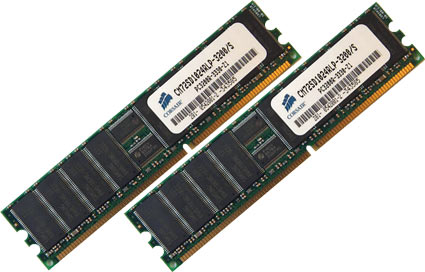
\includegraphics[height=0.75in]{cram}
  \end{center}

  \begin{itemize}
    \item In reality, databases do not contain every possible tuple.
    \item How do we store arbitrary relations classically?
    \item A RAM with $a$-bit addresses and $d$-bit data words
          can store an arbitrary relation on bits:
    \begin{itemize}
      \item Up to arity $d$
      \item Up to $2^a$ tuples.
    \end{itemize}
    \item To get efficient algorithms, we assume constant-time access.
  \end{itemize}
}

%------------------------------------------------------------------------------
\frame[label=qram-hybrid]{

  \frametitle{Quantum-Classical Hybrid Model}

  Any practical model must combine classical and quantum computation.

  \vspace{0.5\baselineskip}

  \begin{center}
  \begin{tabular}{|l|c|l|}
  \textbf{Classical Computer} & $\Rightarrow $ & \textbf{Quantum Computer}\\
   & Program description &\\
  Deterministic control &  & Quantum operations\\
  User interfaces       &  &\\
  Hard drive storage    & Measurement values  & \\
  Normal binary states  & $\Leftarrow $ & Quantum state
  \end{tabular}
  \end{center}
}

%------------------------------------------------------------------------------
\frame[label=qram-circuit]{

  \frametitle{Quantum Random Access Memory (QRAM)}

  A quantum RAM with $a$-bit addresses and $d$-bit data
  words has classical lines for reading and writing and
  quantum lines for the search algorithm.

  Classical data is encoded into qubits. Addresses can mixed,
  and the output is mixed data associated (\textbf{entangled}) with
  the addresses.

  \begin{center}
  \footnotesize
  \begin{tabular}{l|c|l}
    \hline
    $\ket{a_1}$ & & $\ket{a_1,d_1}$\\
    $\ket{a_2}$ & & \\
    $\ket{a_3}$ & & $\ket{a_2,d_2}$\\
    $\ket{r_1}$ & &\\
    $\ket{r_2}$ & \textbf{QRAM} & $\ket{a_3,d_3}$\\
    $\ket{r_3}$ & &\\
    $\ket{d_1}$ & & $\ket{d_1}$\\
    $\ket{d_2}$ & & $\ket{d_2}$\\
    $\ket{d_3}$ & & $\ket{d_3}$\\
    \hline
  \end{tabular}
  \normalsize
  \end{center}

}

%------------------------------------------------------------------------------
\frame[label=qram-grover]{

  \frametitle{Generalized Grover}

  What do we have to change in Grover's algorithm?

  \begin{enumerate}
  \item \textbf{Begin by reading the database mix state $\ket{D}$.}
  \item For each Grover iteration:
  \begin{enumerate}
  \item Query the oracle function $f$ as before.
  \item \textbf{Flip the marked states about the unmarked states as before.}
  \item Flip all states about $\ket{D}$.
  \end{enumerate}
  \item Measure the register.
  \end{enumerate}

  \begin{itemize}
  \item Grover's oracle $f$ is a black box, which we can ``fill in''.
  \item We can design an $f$ for many relational operations.
  \end{itemize}

}

%%%%%%%%%%%%%%%%%%%%%%%%%%%%%%%%%%%%%%%%%%%%%%%%%%%%%%%%%%%%%%%%%%%%%%%%%%%%%%%
\section{Algorithms}

%------------------------------------------------------------------------------
\frame[label=alg-ss]{

  \frametitle{Subset Search Example}

   \footnotesize
   \begin{center}
    \begin{tabular}{|l|l|}
      \hline
      \textbf{Item ID} & \textbf{Group ID}\\
      \hline
       Al Gore & Wikipedia\\ \hline
       Al Gore & Rotten Tomatoes\\ \hline
       Al Gore & whitehouse.gov\\ \hline
       Democrats & whitehouse.gov\\ \hline
       Democrats & Wikipedia\\ \hline
       Global warming & Nature\\ \hline
       Global warming & Rotten Tomatoes\\
      \hline
    \end{tabular}

   \vspace{\baselineskip}

    \textbf{Searched Subset}\\
    \begin{tabular}{|l|}
    \hline
      Al Gore \\ \hline
      Global warming\\ \hline
    \end{tabular}\\

   \vspace{\baselineskip}

    \textbf{Result}\\
    \begin{tabular}{|l|}
    \hline
      Rotten Tomatoes\\ \hline
    \end{tabular}
  \end{center}
  \normalsize

}

%------------------------------------------------------------------------------
\frame[label=alg-ss-2]{

  \frametitle{Subset Search Bounds}

   You are given:
   \begin{itemize}
     \item A table $G$ of $g$ group IDs.
     \item A table $I$ of $N$ items with foreign keys into $I$.
   \end{itemize}

   How to find all groups containing a particular subset of $k$ items?

   \textbf{Approach:} Store an $N$-bit vector with each of $g$ group IDs.
   Each bit is 1 if the corresponding item belongs to that group and
   0 otherwise. $f$ ANDs the item bits restricted to the
   subset.

   \vspace{0.5\baselineskip}

   \begin{itemize}
     \item Classical: $O(gk)$ time, $O(gN)$ space.
     \item Quantum: $O(g\sqrt{kt})$ time, $O(gN)$ space.
   \end{itemize}

   \vspace{0.5\baselineskip}

   \textbf{Applications:} web search, feature tagging databases.
}

%------------------------------------------------------------------------------
\frame[label=alg-nn]{

  \frametitle{Nearest Neighbor Example}

   \footnotesize
   \textbf{Database}
   \begin{tabular}{|l|l|l|l|l|l|l|}
   \hline
   \textbf{Name} & \textbf{Tall} & \textbf{Funny} & \textbf{Super} &
                   \textbf{Famous} & \textbf{Genius} & \textbf{Fictional} \\
   \hline
   Clark Kent  & Yes & No  & Yes & No  & No & Yes\\ \hline
   Jon Stewart & No  & Yes & No  & Yes & No & No\\ \hline
   Stephen Hawking & No & No & No & Yes & Yes & No\\ \hline
   \end{tabular}

   \vspace{0.5\baselineskip}

   \textbf{Query}
   \begin{tabular}{|l|l|l|l|l|l|}
   \hline
   \textbf{Tall} & \textbf{Funny} & \textbf{Super} &
                   \textbf{Famous} & \textbf{Genius} & \textbf{Fictional} \\
   \hline
   Don't care & Yes & Yes & Don't care & Don't care & No\\ \hline
   \end{tabular}

   \vspace{0.5\baselineskip}

   \textbf{Result}
   \begin{tabular}{|l|}
   \hline
   \textbf{Name}\\ \hline
   Jon Stewart \\ \hline
   \end{tabular}
   \normalsize

   \vspace{0.5\baselineskip}

   You are given:
   \begin{itemize}
     \item A table $N$ tuples, each with $k$ binary attributes.
   \end{itemize}

   \vspace{0.5\baselineskip}

   How do you find the ``neighbor'' with the fewest differences from
   a particular input tuple?
}

%------------------------------------------------------------------------------
\frame[label=alg-nn-2]{

  \frametitle{Nearest Neighbor Bounds}

   \textbf{Approach:} $f$ computes the Hamming distance restricted to
   fields we care about. Then use quantum search on the distances to
   find the minimum [DH96].

   \vspace{0.5\baselineskip}

   \begin{itemize}
     \item Classical: $d\log{N}/\min{(\epsilon^2,1)}$ update and query time,
$N^{O(1/\epsilon^2 + \log{(1+\epsilon)}/(1+\epsilon))}$ space [HIM03].
     \item Quantum: $O(d\sqrt{N}))$ query time, $O(1)$ update time, $O(1)$ space.
   \end{itemize}

   \vspace{0.5\baselineskip}

   \textbf{Applications:} machine learning, probabilistic databases.
}

%%%%%%%%%%%%%%%%%%%%%%%%%%%%%%%%%%%%%%%%%%%%%%%%%%%%%%%%%%%%%%%%%%%%%%%%%%%%%%%
\section{Future}

%------------------------------------------------------------------------------
\frame[label=future-skepticism]{

  \frametitle{Skepticism}

  \begin{itemize}
    \item Will cheap, fast QRAMs ever be feasible?
      \begin{itemize}
        \item Not without compelling applications.
      \end{itemize}
    \item Don't classical databases already scale for realistic datasets?
      \begin{itemize}
        \item Not for future quantum data
              (entangled crypto qubits, intermediate computation, quantum software).
        \item Most classical applications did not exist before the technology
              (bootstrapping problem).
      \end{itemize}
  \end{itemize}
}

%------------------------------------------------------------------------------
\frame[label=future-work]{

  \frametitle{Future Work}

  \begin{itemize}
    \item
    Do aggregation with quantum counting.
    \item 
    Use quantum data structures or complex amplitudes
    to improve upper bounds given.
    \item
    Find an efficient quantum join (naively in $O(N^{3/2})$, 
    must beat classical $O(N\log{N})$).
    \item
    Combine with the Quantum Fourier transform to do search on
    2D images, video, audio, etc.
  \end{itemize}
}

\end{document}



%%% Local Variables: 
%%% mode: latex
%%% TeX-master: "beamerexample2.article"
%%% End: 
